% Mau nhap: khong can ma ID6; chon dang va muc do khi duyet.
\documentclass{article}
\usepackage{tikz,amsmath}
\begin{document}
\begin{ex}
Gieo một xúc xắc cân đối. Xác suất xuất hiện số chấm chẵn là bao nhiêu?
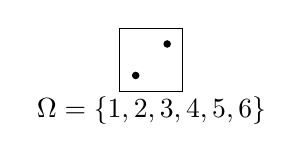
\begin{tikzpicture}[scale=0.8]
  \draw (0,0) rectangle (1,1);
  \fill (0.25,0.25) circle (0.06);
  \fill (0.75,0.75) circle (0.06);
  \node at (0.5,-0.3) {$\Omega=\{1,2,3,4,5,6\}$};
\end{tikzpicture}
\choice{\True $\frac{1}{2}$}{$\frac{1}{3}$}{$\frac{1}{6}$}{$1$}
\loigiai{Có ba số chẵn trong sáu kết quả đồng khả năng nên $P=\frac{3}{6}=\frac{1}{2}$.}
\end{ex}

\begin{ex}
Gieo một xúc xắc cân đối. Xét các phát biểu sau.
\choiceTF{\True Không gian mẫu có 6 phần tử.}{Không gian mẫu có 2 phần tử.}{\True Có 3 kết quả là số chẵn.}{Số chấm luôn bằng 6.}
\loigiai{Các kết quả có thể xảy ra là 1, 2, 3, 4, 5, 6.}
\end{ex}

\begin{ex}
Bảng ghi số viên bi theo màu. Lấy ngẫu nhiên một viên. Tính xác suất lấy được viên bi thuộc nhóm A.
\begin{tabular}{|c|c|}
\hline A & B \\ \hline 3 & 3 \\ \hline
\end{tabular}
\shortans{0.5}
\loigiai{Xác suất bằng $\frac{3}{3+3}=0.5$.}
\end{ex}
\end{document}
